\documentclass{article}
\usepackage[utf8]{inputenc}
\title{Lecture 11: feature learning, neural nets and back propitiation}
\author{wbg231 }
\date{December 2022}
\newcommand{\R}{$\mathbb{R}$}
\newcommand{\B}{$\beta$}
\newcommand{\A}{$\alpha$}
\newcommand{\D}{\Delta}

\newcommand{\avector}[2]{(#1_2,\ldots,#1_{#2})}
\newcommand{\makedef}[2]{$\textbf{#1}$:#2 }
\usepackage{tikz,graphicx,hyperref,amsmath,amsfonts,amscd,amssymb,bm,cite,epsfig,epsf,url}

\begin{document}

\maketitle

\section*{introduction}
\begin{itemize}
\item neural networks have empirical sauces but poor theoretical understanding 
\item how do you learn them from scratch 
\item one of the key ideas is representation learning 
\item here we want to be able to learn a representation as opposed to explicitly giving a kernel as we have done in the past. 
\item we want to be able to learn the feature space
\item learning back propagation which allows us to calculate the gradient and conduct SGD to optimize
\section{feature engineering}
\item many problems are non linear 
\item one method is to express the non linear models in a linear form $$f(x)=w^t\phi(X)$$ where $\phi$ is a feature map mapping from our input space to feature space. 
\item note that this model is linear in $\phi(x)$ not x. 
\item for $\phi$ we can use a feature map that defines a kernel such as polynomials 
\subsection{problem decomposition}
\item suppose we want to predict how popular a restaurant is given some features, like we are building yelp or google maps. 
\item we want to be able to recommend the restaurant to the users 
\item have raw features: number of dishes , price of dish number of seats, size of restaurants. wine quality.
\item we can decompose the problem into many subproblems for example 
\begin{itemize}
    \item h1(number of dishes, wine quality) = food quality
    \item h2(zip code)= walk ability
    \item etc
\end{itemize}
\item each intermediate model can sovle a subproblem. 
\item so we have many indepent models that each try to predict there own task 
\item then we can finally have a weighted linear modll that takes each of the intermediate probelms to make a finaly prediction. $h(\text{all featres}=w_1*\text{food quality}+w_2*\text{walk ability} +\Sigma_{i=1}^{n}w_ih_i(x_i)$
\item this is kinda like feature engeneering we define the meaningfull atirbutes as the features then use those features to make a linear model that allows us to predict the final quantity we want 
\item neural nets are good at learning these intermediate features, maybe not those that would be intrepertiable to us, but prolly oones that are predictive
\subsection{perceptrons as logic gates}
\item recall the perceptron algorithm \\ 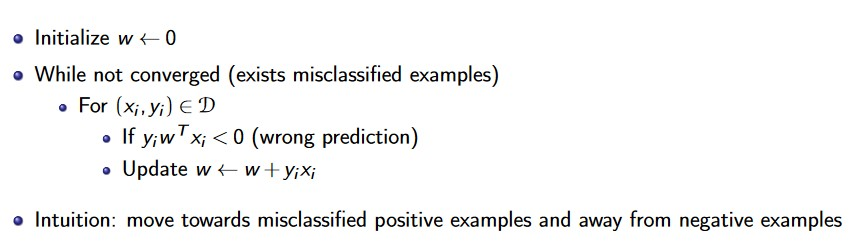
\includegraphics[width=10cm]{lecture_notes/lecture_11/immages/l11_1.jpg}
\item more or less the goal is we are iterative trying to learn separating hyperplane between two linearly separable sets of data
\item 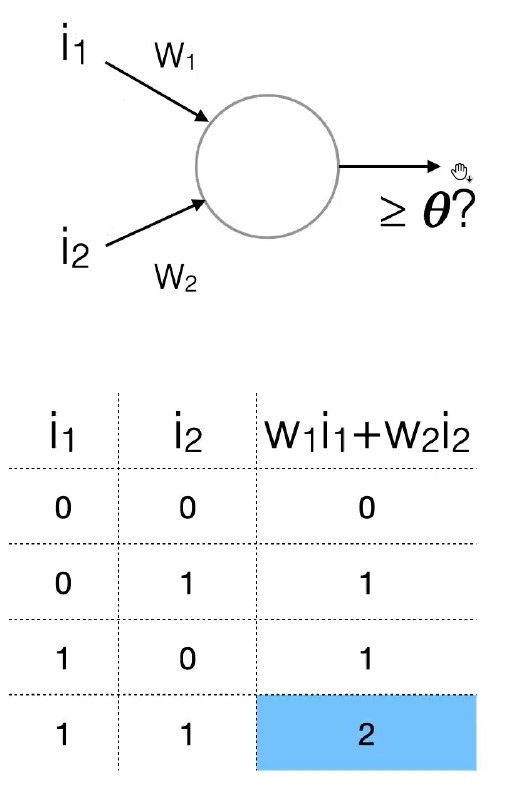
\includegraphics[width=10cm]{lecture_notes/lecture_11/immages/l11_2.jpg}
\item so the input's are all the i's and the output is taking a weighted sum of these i's then see if the dot product is above theta and if so output 1 and otherwise output zero
\item so in this case think of our task as input $i\in \matbb{R}^{2}$ and weight vector $w\in\mathbb{R}^2$ with threshold $\theta \in \mathbb{R}$
we predict as $\mathbb{I}(w^ti\geq \theta)$
\item this implements a logic gate and operation if $i_1, i_2$ are bianry, and $w_1, w_2=1$ and $\theta=1$
\subsection{limiations}
\item this can build and as well as or gates but it Can not build xor (ie just 1) or xnor (ie both or neither)   
\item we can not use a perceptron to do this, as there is no linear boundary between these nodes. 
\subsection{multi layer perceptron }
\item we can however do this with a multi-lear perceptron 
\item we add what are call hidden nodes these h layer. 
\item so compuation is the same as before, h1 nad h2 take some weighed sum of our input then our output is a wieghted sum of h1 and h2,
\item each h1 and h2 are threshold unctiosn taht only fire if the combination fo there inpuuts are above a certain threshold. \\
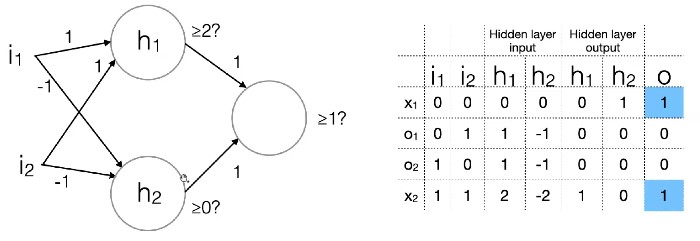
\includegraphics[width=10cm]{lecture_notes/lecture_11/immages/l11_3.jpg}
\item so this is a nor gate.
\item you can view the hidden node as a feature map, it is a bassicaly taking $x\rightarrow \phi(x)$ that is it is repsenitng out inputs in a new space such that they are now linerly seperabale, allowing the nueal new to solve this problem 
\item 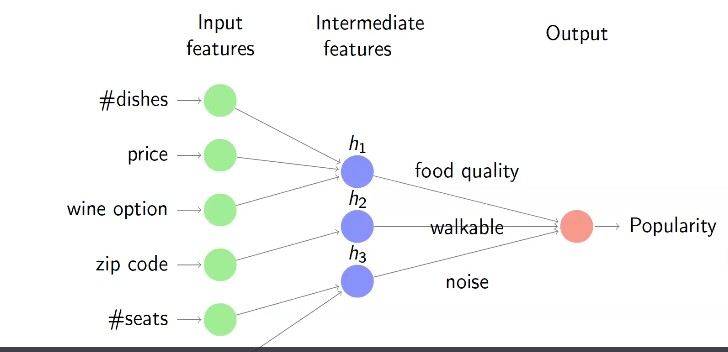
\includegraphics[width=10cm]{lecture_notes/lecture_11/immages/l11_4.jpg}
\item in a nuearl network case we do not know what the hidden feautre is we are inistead learing the featres as we go
\subsection{nuearl networks}
\item the key idea is to learn intermediate features 
\item \textbf{feature engeneering} manually specficy $\phi(X)$ base don domain knowledge and the learn the weights $$f(x)=w^t\phi(x)$$
\item \textbf{feature leanring } learn both the featurers (K hidden units) and the weights $$h(x)=[h_1(x)\cdots h_k(x)]$$
$$f(x)=w^th(X)$$
\item nuearl nets are about feature learning 
\subsection{feature leanring example}
\item a feature conves over the immages and lookes for the higest pattern match 
\item trdaitonally people use gabor filters or otehr image feature extracts and an svm for image classficaiton (this is feature extaction)
\item neuarly networks take ini images and learn teh filters that are most usefull for solving the taks. this is likely more efecintent then explicitly engender feature maps 
\subsection{inspiration : the brain }
\item our brains has about 100 billion neurons each of which communicate tot the other 1000 neurons with non-linear computations. 
\item neurons receive input signals and accumulate voltage after some threshold they will fire stiring response 
\subsection{activation function}
\item we can model a simpler computation by an activatian function 
\item this function apples a non-linearity on the inputs and fires after some threshold 
$$h_i(x)=\sigma(v_i^tx)$$ so that is we pat the dot product of some vector $v_i$ and the input through the a function to get the output of our hidden layer 
\item there are a number of possible activation functions 
\item in the classic perceptron it is the sign function ie $\mathbb{I}(v_i^x\geq 0)$ this is non differentiable
\item we can use a diferntibale aproxiamtion like teh sigmoid funciton, or hyperbolic trangnet function 
\item tow later nuearl network (have one hidden layer and one output layer ) can be writen as $$f(x)=\Sigma_{k=1}^{K}w_{k}h_{k}(x)$$ so this means the network is 2 layers deep and k layers wide (ie it has one hidden layer that learns k possible features) then the final output is a weighted combination of those k possible features.  \\
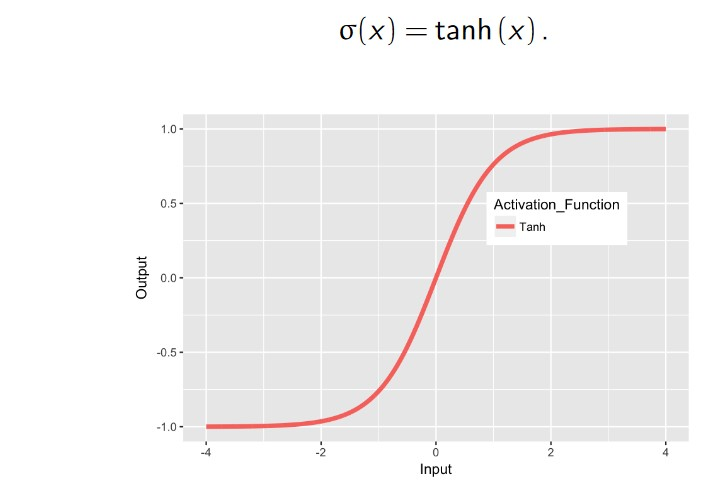
\includegraphics[width=10cm]{lecture_notes/lecture_11/immages/l11_5.jpg}
\item this is the hyperbolic tangent function 
\item this has a problem called the \href{https://en.wikipedia.org/wiki/Vanishing_gradient_problem}{vanishing gradient problem}, in which basically you can see how the gradients drop off exponentially so as we add more hidden layers ie pass our inputs through more of these, the gradients shrink over time 

\subsection{activation functions }
\item more recently a populor activation function is the \textbf{rectifies linear (ReLU) function } which has been very popular $$\phi(x)=max(0,x)$$
\item this function fires linearly passed 0 and does not fire before it so it has a simple derivative everywhere
\\
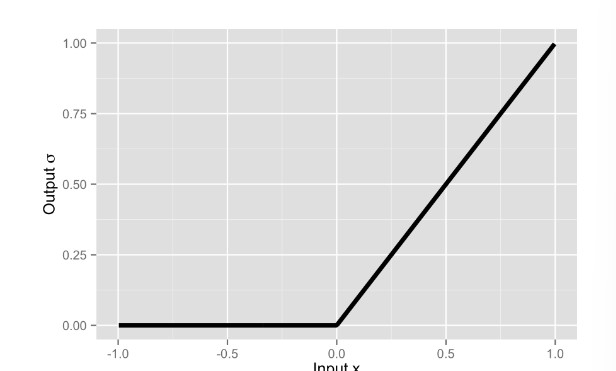
\includegraphics[width=10cm]{lecture_notes/lecture_11/immages/l11_6.jpg}
\subsection{aproximation ability}
\item consider a nueral net of the form $$f(x)=w^th(x)=w^t\sigma(v^tx)$$ where $w\in \mathbb{R}^{3}$ and $h\in \mathbb{R}^3$ that is it is one layer deep and 3 layers wide with $\sigma=tanh(x)$
\item 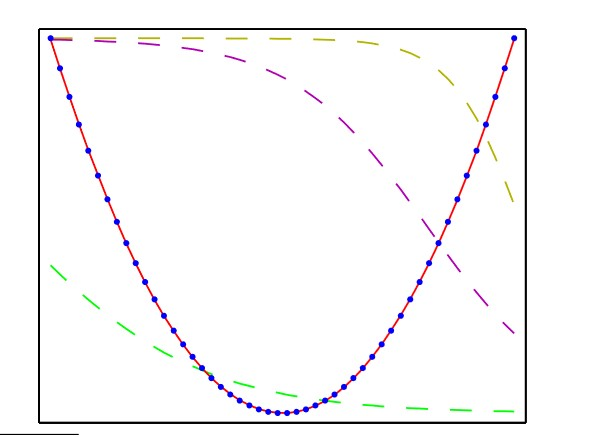
\includegraphics[width=10cm]{lecture_notes/lecture_11/immages/l11_7.jpg}
\item the blue dots are triaing points 
\item the dashed lines are our hidden layers outputs and the final output is in red 
\item we did a really good job learning a quadratic function 
\subsection{example 2 }
\item suppose we have the same set up and want to learn $f(x)=sin(x)$
\item 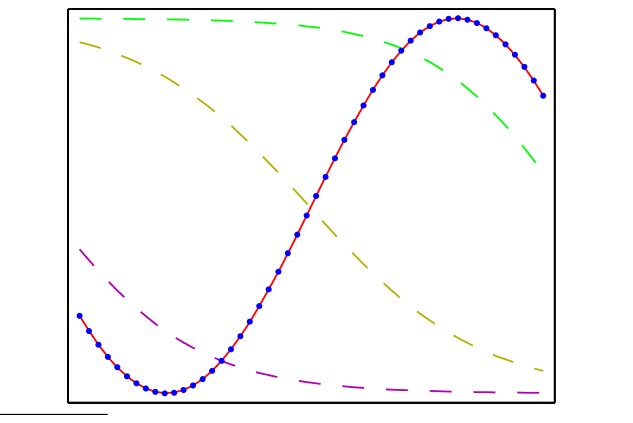
\includegraphics[width=10cm]{lecture_notes/lecture_11/immages/l11_8.jpg}
\item we are also able to lose this fucntion well 
\item so recall that our set up is this $$f(x)=\Sigma_{k=1}^{k}w_k^th_k(x)=\Sigma_{k=1}^{k}w_k\sigma(v^tx)$$ where $w\in \mathbb{R}^{3}$ and $h\in \mathbb{R}^3$
\item so we are learning k hidden weights $v_k\in \mathbb{R}^{n}$ which weight each of our inputs that is then passn to the actvation fucntion 
\item then we are learning one output weight $w\in \mahtbb^{3}$ which weights our 3 learned activation fcuntions 
\subsection{aproximation ability absolute value}
\item so suppose we are trying to learn $f(x)=|x|$
\item 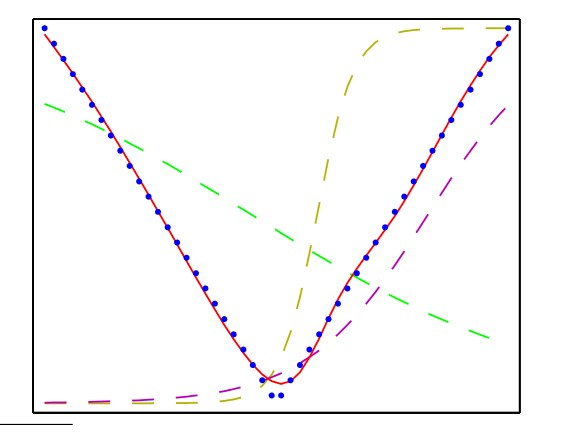
\includegraphics[width=10cm]{lecture_notes/lecture_11/immages/l11_9.jpg}
\item so we have a bit of trouble learning the the point where f(x) is non-diferntiable in this case 
\subsection{universal approximate theorem}
\item \textbf{universal approximate theorem} A nearly network with one possibly huge hidden layer $\hat{F}(x)$ can approximate any continuous function $F(x)$ on a closed and bounded subset of $\mathbb{R}^d$ under mild assumptions on the activation function $\forall \epsilon>0$ there exists an integer N such that $$\hat{F}(x)=\Sigma_{i=1}^{N}w_i\sigma(v_i^Tx+b_i)$$ satisfies $$|\hat{F}(x)-F(x)|<\epsilon$$

\item this is really just saying that given an arbitrarily wide neural network we can approximate any continuous function f that is continuous on a closed interval S (ie let S define $S\subset \mathbb{R}^D$ we must have $\forall c\in S  \forall \epsilon>0\quad \exists \delta>0$ such that whenever $X\in S$ and $|x-c|<\delta \Rightarrow |f(x)-f(c)|\leq \epsilon$ that is simply at all points on our interval our function has a finite rate of change) 
\item there are a lot of papers that go into proving this idk how use full it will be but here is a link to look into \href{https://ai.stackexchange.com/questions/13317/where-can-i-find-the-proof-of-the-universal-approximation-theorem}{stack overflow discussion}
\item for the theorem to work the number of hidden units needs to be exponential in d. that is if we have $x\in \mahtbb{R}^d$ our number of hidden units must be $\geq 2^d$ (so just having a super wide one layer nn does not scale)
\item the theorem does not tell us how to learn these parameters just that they exists 
\item it does not tell us from a practical perspective why this works well or how to build them 
\subsection{Deep neural nets}
\item in practice we get around this by building deeper not wider neural nets 
\item wider means more hidden units (in each layer)
\itme deep means more hidden layers
\item 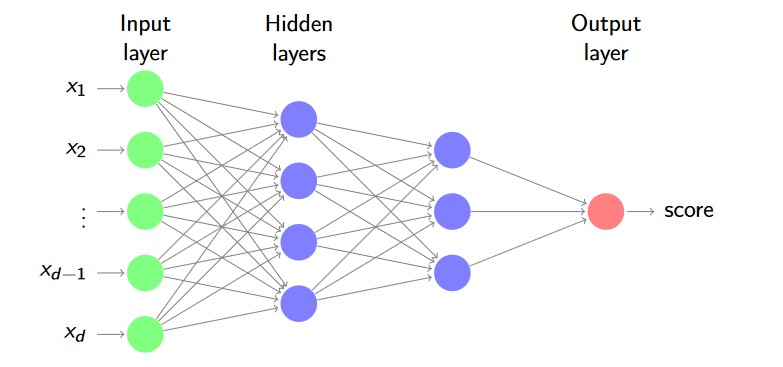
\includegraphics[widht=10cm]{lecture_notes/lecture_11/immages/l11_10.jpg}
\subsection{multi layer perception formal definition}
\item input space $X=\mathbb{R}^D$
\item action space $A=\mathbb{R}^K$ (assuming we have a k class classification problem that is we are outputting a k dimensional vector of scores)
\item let $\sigma \rightarrow \mathbb{R}\rightarrow \mathbb{R}$ be an activation function (it could tanh or ReLU)
\item let us consider an MLP of L hidden layers with each hidden layer having m hidden units 
\item the first hidden layer is given by $$h^{1}(x)=\Sigma(W^1x+b^1)$$
for parameters $W^1\in \mathbb{R}^{m\times d}$ and $b^1\in \mathbb{R}^m$ and $\sigma$ is applied to each entry of its argument 
\item each subsequent hidden layer takes the output $o\in \mathbb{R}^m$ of the previous layer and produces $$h^{j}(o^{j-1})=\sigma(W^jo^{j-1}+b^j). \forall j \in [2,L]$$ where $w^{j}\in \mahtbb{R}^{m\times m}, b^j\in \mathbb{R}^m$
\item and let the last later be an affine mapping ie no activation function $$a(o^l)=W^{l+1}O^L+b^{l+1}$$ where $W^{l+1}\in \mathbb{R}^{k\times m}$ and $b^{l+1}\in \mathbb{R}^{k}$
\item the full neural network is given by a composition of layers $$f(x)=(a\circ h^L\circ \cdots \circ h^1)(x)$$
\item typically the last layer gives us a score that we can use for regression or classification 
\item so your first layer takes your input features $in \mathbb{R}^{d}$. then learns M new features each of which are a weighted linear combination of the d original inputs. so in total you are learning $W\in \mathbb{R}^{m\times d}$ weights this produces m feature scores that are then passed through our action fucntion to get out output for that layer $o\in \mathbb{R}^m$
\item then at each subsequent hidden layer we take the m learned outputs learn m new features that are some linear combinatoon of those m features, and pass thsoe through our activation function 
\item finally at the output layer we are given our $o^{L}\in \mathbb{R}^m$ that is the m scores of our last hidedn layer, we then weight each of these m outputs to produce 1 of the k final dimensions resulting in out final output $y\in \mathbb{R}^{k}$ note that at this stage we are not applying the activation fcunton we are just taking some weighted combination fo our learned features as output. 
\subsection{classification}
\item for each x we can compute a linear score function of each class that is $$x\rightarrow (<w_1,x>\cdots <w_k,x>)\in \mathbb{R}^{k}$$ 
\item then we use some function to map this vectors into a probability vector $\theta$
\item in multinomial logistic regression we used the softmax
\item teh softmax maps scores $s=(s_1\cdots s_k)$ to a catagorical distrobution$$ (s_1,\cdots , s_k)\rightarrow \theta = softmax(s_1\cdots s_k)=(\frac{e^s1}{\Sigma_{i=1}^{k}e^s_i},\cdots, \frac{e^sk}{\Sigma_{i=1}^{k}e^s_i}  )$$
this more or less maps each score to a normalized value, such that all of them sum to one and thus they are a probability vector representing the likelihood of the input being each class .
\subsection{nonlinear generalization of matrimonial logistic regression}
\item from each x we compute a non-linear  score function for each class $$x\rightarrow (f_1(x)\cdots f_k(x))$$
where $f_i(x)$ are the output of the final hidden layer of the neural network 
\item leaning maximize the log likelihood of training data. $$argmax_{f_1\cdots f_k}\Sigma_{i=1}^{n}log[softmax(f_1(x_i)\cdots f_k(x_i))]$$
\item so more or less we use the hidden layers of our nn to get some optimal feature map 
\item we then use our output layer of the nn to get a weighted score function of these features, 
\item we then run use MLE to max the log likelihood of the sift max of our training data. 
\subsection{interim discussion}
\itme with the right representations we can turn non-linear problems into linear ones 
\itme the goal of representaiton leanring is to automatically discover usefull features from raw data 
\item the building blocks of this are 
\begin{enumerate}
    \item input layers whcih are non learnable parameraters
    \item hidden layers whcih are affine combinations of features passed through non-linear afcativion function 
    \item then the outout layer whcih is an affine combination of our final hidden layer pased through teh soft max 
\end{enumerate}
\item a single potentially huge hidden layer is sufficent to aproximate any fucntion 
\item how ever in practice it is more effiecnt to train multiple hidden layers
\subsection{fitting the parameters of an MLP}
\item input space $X=\mathbb{R}^{d}$
\item assume this is a regression problem so our output and action space are both $A=Y=\mathbb{R}$
\item consider the hypothesis space of MLP with one hidden layer with 3 nodes. $$f(X)=w_{0}+w_{1}h_{1}(x)+w_{2}h_{2}(x)+w_{3}h_{3}(x)$$
where $$h_{i}(x)=\sigma(v_ix+b_i)\forall i\in [1,3]$$ for fixed activation function $\sigma  \mathbb{R}\rightarrow \mathbb{R}$
\item we need to fit 10 parameters $b_1,b_2,b_3,b_1,v_2,v_3, w_0,w_1,w_2,w_2\mathbb{R}$

\subsection{finding the best hyperparameters}
\item our hypothesis space is linear functions $\theta = (b_1,b_2,b_3,b_1,v_2,v_3, w_0,w_1,w_2,w_2) \in \Theta=\mathbb{R}^{10}$
\item we are using erm so for the training set our goal is to find $$\hat{\theta}=\argmin_{\theta\in \mathbb{R}^{10}}\frac{1}{N}\Sigma_{i=1}^{n}(f(x_i,\theta)-y_i)^2$$
\item suppose that we are fixing our prediction function to be $$f(x)=w_0+\Sigma_{i=1}^{3}tanh(v_ix+b_i)$$
\item is this function differentiable with respect to $\theta$? yeah $\frac{d}{dx}(tanh(x))=1-tanh(x)^2$
\item is our loss function convex? than is not convex, and the composition of convex functions is not necessarily convex. so we don't know 
\item so we might get local minimums
\section{back propagation}
\subsection{gradient descent for large nn}
\item mathematically can do this as normal with partial derivatives, but that would be time consuming and error prone for large networks
\item \textcolor{blue}{back propagation} computes gradients for nu earl networks in a systematic and efficient way
\item can be visualized nicely with computation graphs that expose to structure of computation both in terms of \textcolor{green}{modality and dependency}
\subsection{functions as nodes in a graph}
\item think of each computation of a neural network as a node that takes a set of inputs and produces a set of outputs
\item this can be presented in either of the following ways\\ 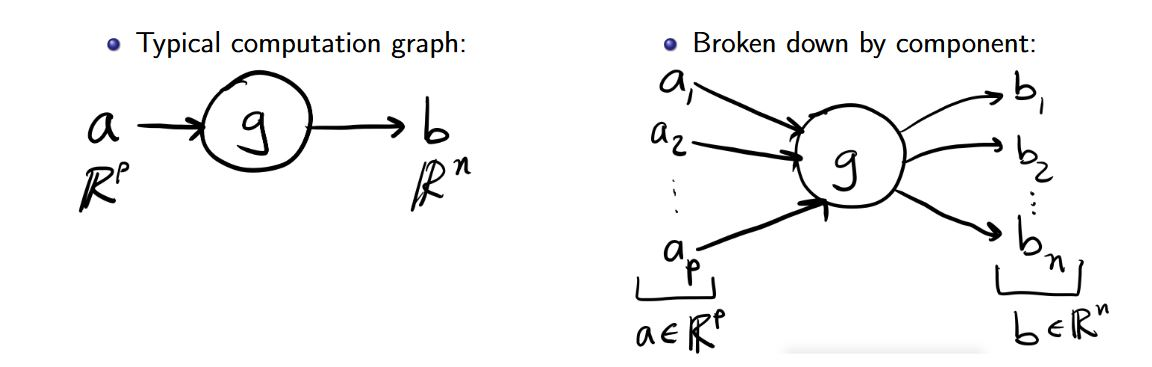
\includegraphics[width=10cm]{lecture_notes/lecture_11/immages/l11_11.JPG}
\subsection{partial derivatives of an affine function }
\item an \textcolor{red}{affine function} is an function $f(x)=Ax+c: A\in \mathbb{R}^{n\times d}, x\in \mathbb{R}^{d}, c\in \mathb{R}^{n}$ that is a function that is a linear combination plus adding a constant 
\item consider the affine function $g(x)=Mx+c: M\in \mathbb{R}^{n\times p}$ and $c\in \mathbb{R}^{n}$
\item let $b=g(a)=Ma+c$ we can see that $$b_i=\Sigma_{j=1}^{p}M_{i,j}x_{j}+c_{i}$$
\item suppose $x_k\leftarrow x_k+\delta$ what does this make $b_i$?
$$b_i=\Sigma_{j=1}^{p}M_{i,j}x_{j}+c_{i}=b_i=\Sigma_{j\neq k}M_{i,j}x_{j}+M_{i,k}(x_{k}+\delta)+c_{i}=b_i+M_{i,k}\delta$$
\item recall that the partial derivative $\frac{\partial b_i}{\partial a_j}$ is the rate of change of $b_i$ wrt to $a_j$ 
\item so if we make a small change to $a_j$ such that $a_j\leftarrow a_j+\delta$
\item then for small $\delta$ we have  $b_i\approx b_i+\frac{\partial b_i}{\partial a_i}\delta$ this is a Taylor approximation 
\item suppose we have $g:\mathbb{R}^{p}\rightarrow \mathbb{R}^{n}$ and $f:\mathbb{R}^{n}\rightarrow \mathbb{R}^{m}$ where $b=g(a)$ and $c=f(b)$ we can visualize this as \\ 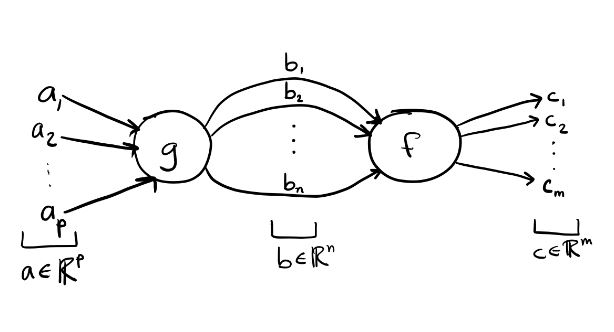
\includegraphics[width=10cm]{lecture_notes/lecture_11/immages/l11_12.JPG}
\item what is the effect of a small change in $a_j$ on $c_i$? by the chain rule it is $$\frac{\partial c_i}{\partial a_j}=\frac{\partial f(b)}{\partial a_j}=\frac{\partial f(g(a))}{\partial a_j}=\frac{\partial f(b)}{\partial g(a)}\frac{\partial g(a)}{\partial a_i}=\Sigma_{k=1}^{p}\frac{\partial f(b)}{\partial g(a_k)}\frac{\partial g(a_k)}{\partial a_i}$$
\subsection{example linear least square}
\item let our hypothesis space be $$\mathcal{H}=\{f(x)=x^t+b:w\in \mathbb{R}^d, b\in \mathbb{R}\}$$
\item let our data set be $$\mathcal{D}=((x_1_y_1), \cdots (x_n,y_n)\in \mathbb{R}^{n\times d}$$ (keep in mind here that $(. , .  )$ is a bag ie order matters, and there can be repeated elements and $\{\}$ are sets where order does not matter and there are no repeated elements
\item let our loss function be least squares that is $$\ell_i(w,b)=((f(w, b, x_i)- y_i))^2=(w^tx_i+b- y_i)^2$$
\item in sgd each round we chose a random training instance $i\in [1,n]$ and take gradient step $$w_j\leftarrow w_j-\eta \frac{\partial \ell_{i}(w,b)}{\partial w_j} \forall j\in [1,d]$$ $$b\leftarrow b- \eta \frac{\partial \ell_i(w,b)}{\partial b}$$ That is we adjust each element of the weight vector and bias term in the direction that minimizes our loss function with respect to training example i at each step for a given step size $\eta > 0$
\item  we make prediction $\hat{y}=f(x,w,b)=\Sigma_{j=1}_{j=1}^{d}w_jx_j+b=w^tx+b$
\item our residual is $r=y-\hat{y}$
\item our loss function is $\ell(w,b)=(w^tx+b-y)^2=(\hat{y}-y)^2=r^2$
\item we can visualize this as \\ 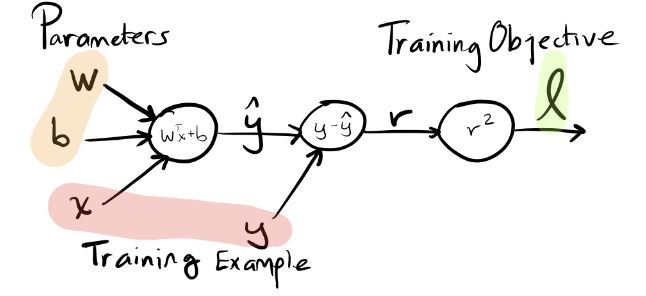
\includegraphics[width=10cm]{lecture_notes/lecture_11/immages/l11_13.JPG}
\item so lets work our way from the output $\ell$ back to the parameters $w,b$ reusing previous computations as needed 
\item the partial of loss with respect to residual is $\frac{\partial \ell}{\partial r}=2r$
\item the partial of loss with respect to y is $\frac{\partial \ell}{\partial \hat{y}}=\frac{\partial \ell}{\partial r(\hat{y}})*\frac{\partial r(\hat{y})}{\partial \hat{y}}=2r*\frac{\partial }{\partial \hat{y}} (y-\hat{y})=-2r$
\item $\frac{\partial \ell }{\partial b}=\frac{\partial \ell}{\partial r(\hat{y}})*\frac{\partial r(\hat{y})}{\partial \hat{y}(b)}* \frac{\partial \hat{y}(b)}{\partial b}=-2r(1)=-2r$
\item $\frac{\partial \ell }{\partial w_j}=\frac{\partial \ell}{\partial r(\hat{y}})*\frac{\partial r(\hat{y})}{\partial \hat{y}(w_j)}* \frac{\partial \hat{y}(w_j)}{\partial w_j}=-2r(x_j)$
\subsection{example ridge regression}
\item we can visualize this as \\ 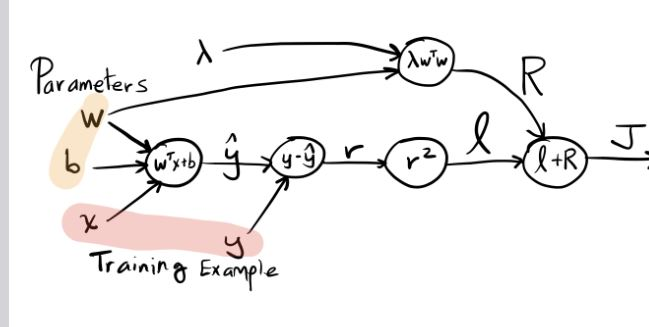
\includegraphics[width=10cm]{lecture_notes/lecture_11/immages/l11_14.JPG}
\item suppose now our objective function was $$j(w,b)=[(w^tx+b)-y]^2+\lambda ||w||_{2}^2$$
\item lets again work backwards 
\item $\frac{\partial j}{\partial r}=\frac{\partial }{\partial r}(r)^2+||w||_{2}^2=2r$
\item $\frac{\partial j}{\partial Y}=\frac{\partial J}{\partial r(Y)}*\frac{\partial r(y)}{\partial\hat{y}}= 2r(-1)=-2r$
\item $\frac{\partial j}{\partial b} = -2r$
\item now the only thing that changes is this $\frac{\partial j}{\partial w_i}=\frac{\parial \ell}{\partial w_i}+\frac{\partial ||w||^{2}_2}{\partial w_i}=-2r(x_j)+2\lambda_iw_i=2(\lambda_iw_i-r(x_i))$
\subsection{overview}
\item learning run gradient descent to find the parameters that minimize our objective function $J$
\item propagation: we compute the gradient with respect to each trainable parameter $\frac{\patial j}{\partial \theta_i}$
\item there are two steps 
\item \textcolor{red }{forward pass} compute intermediate unction value ie the output at each node 
\item \textcolor{red }{backwards pass} compute the partial derivatives of $j$ wrt to all intermediate variables and model parameters 
\item so the question becomes how do we minimize computation?
\begin{itemize}
    \item \textcolor{red}{path sharing} that is each node caches intermediate results so we do not re do computation 
    \item this is dynamic programming 
\end{itemize}
\subsection{forward pass}
\item we preform a \href{https://en.wikipedia.org/wiki/Topological_sorting}{topological sort} on our graph that is we sort the nodes so that a parent node shows up before all of there descendants
\item then for each node we compute the output given the input (where the input is the output of the parent nodes)
\item so a forward pass at intermediate node (ie not start or end) $f_i, j_j$ looks like \\ 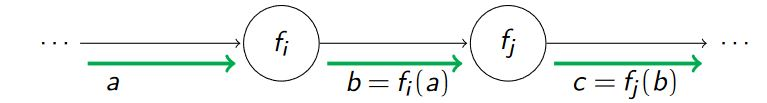
\includegraphics[width=10cm]{lecture_notes/lecture_11/immages/l11_15.JPG}
\item that is we take in some input a calculate the result for that node $f_i(a)$ call that b pass that to the next node $f_j$ calculate the result for that node $f_j(b)=c$ and pass c along 
\subsection{backwards pass }
\item here we order the nodes in reverse topological order that is all descendant nodes must appear before there ancestors 
\item then for each node, we compute the partial derivative of it's output with respect to its input multiplied by the partial derivative of it's children (ie we use the chain rule)
\item so at node $f_i, f_j$ our backwards pass looks like this \\ 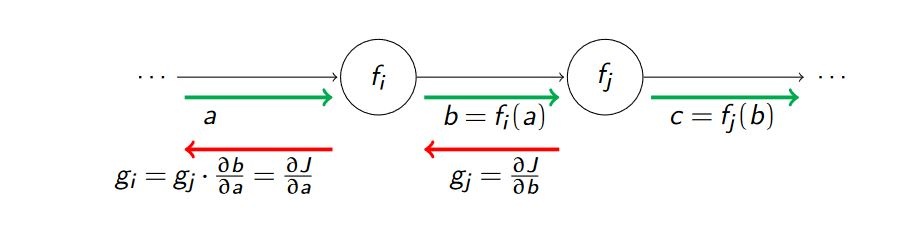
\includegraphics[width=10cm]{lecture_notes/lecture_11/immages/l11_16.JPG}
\subsection{multiple children}
\item suppose we have this case \\ 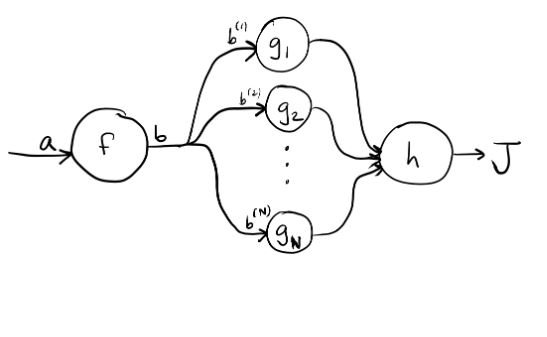
\includegraphics[width=10cm]{lecture_notes/lecture_11/immages/l11_17.JPG}
\item so the forward pass would just be all the intermediate nodes $g_i$ receive $b_i$ and make $g_i$ and pass those to h which passes and makes j
\item the back prop of node $f$ is 
\begin{itemize}
    \item we are given partial derivative $j$ with respect to  all $b_i$ that is $\frac{\partial j}{\partial b_i}$
    \item we output $\frac{\partial j}{\partial b}=\Sigma_{k=1}^{n}\frac{\partial j}{\partial b_K}$ and then $\frac{\partial j}{\partial a}=\frac{\partial j}{\partial b}\frac{\partial b}{\partial a}$

\end{itemize}
\subsection{why backwards}
\item we can writ the gradient in terms of the chain rule let $y=y(c(b(a))$
\item the gradient is $$\frac{\partial y}{\partial a}=(\frac{\partial b}{\partial a}\frac{\partial d}{\partial b})\frac{\partial y}{\partial c}$$
\item it is faster to go go backwards (ie back prop ) since we have a scalar output and vector input
\item forward order could be faster if we have a scalar input and vector output 
\item the optimal order is a matrix chain order problem 
\subsection{ non convex optimization}
\item we could converge to bad local optima, if that the case we want to re run with different initialization 
\item we could hit saddle points, but this rarely happens with SGD and we can use our second derivative test on the found optima to check 
\item there could be regions that are flat ie have low gradient magnitudes so take a long time to train. we could try to get around this with relu activation functions instead of sigmoids
\item if we have the ope site problem and have areas with high curvature that is very large magnitude gradient we could try gradient clipping or having an adaptive step size
\subsection{learning rate}
\item learning rate very important in practice
\item start with a large learning rate and decay towards zero
\item classical theory: convergence is guaranteed for SGD, unless the update step is dominated by a noise term 

\end{itemize}
\end{document}
